
% \begin{quote}
% Markdown Revision 1;\\
% Date: 2018/10/25\\
% Editor: 乔成磊-同济大学,王超锋 Contact:
% qchl0318@163.com,syusuke0516@163.com Updater:
% \href{https://github.com/sjsdfg}{sjsdfg},王超锋
% \end{quote}

\chapter{ 写在前面}\label{ux5199ux5728ux524dux9762}

​
关于训练深度学习模型最难的事情之一是你要处理的参数的数量。无论是从网络本身的层宽(宽度)、层数(深度)、连接方式,还是损失函数的超参数设计和调试,亦或者是学习率、批样本数量、优化器参数等等。这些大量的参数都会有网络模型最终的有效容限直接或者间接的影响。面对如此众多的参数,如果我们要一一对其优化调整,所需的无论是时间、资源都是不切实际。结果证实一些超参数比其它的更为重要,因此认识各个超参数的作用和其可能会造成的影响是深度学习训练中必不可少的一项重要技能。

​
超参数调整可以说是深度学习中理论和实际联系最重要的一个环节。目前,深度学习仍存在很多不可解释的部分,如何设计优化出好的网络可以为深度学习理论的探索提供重要的支持。超参数调整一般分为手动调整和自动优化超参数两种。读者可先浏览思维导图,本章节不会过多阐述所有超参数的详细原理,如果需要了解这部分,您可以翻阅前面的基础章节或者查阅相关文献资料。当然,下面会讲到的一些超参数优化的建议是根据笔者们的实践以及部分文献资料得到认知建议,并不是非常严格且一定有效的,很多研究者可能会很不同意某些的观点或有着不同的直觉,这都是可保留讨论的,因为这很依赖于数据本身情况。

\begin{figure}
\centering
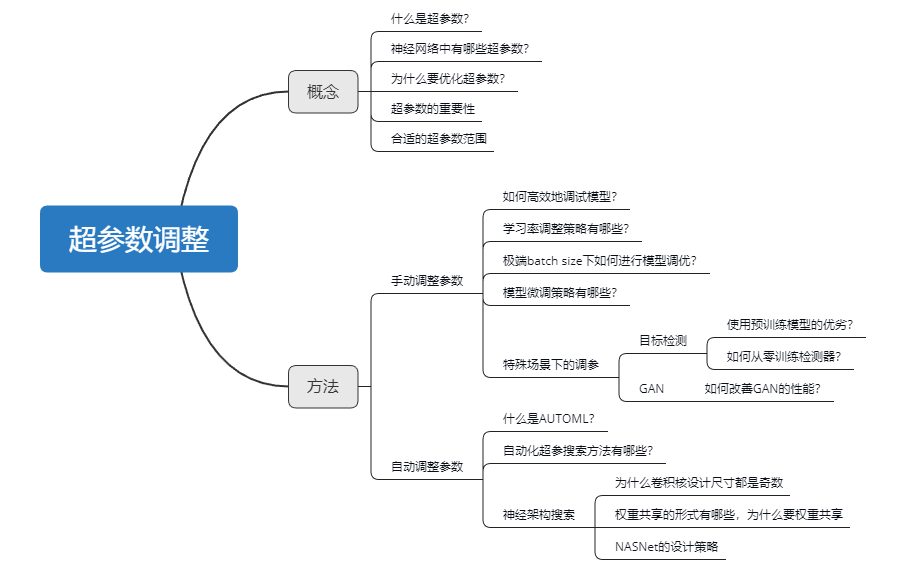
\includegraphics{./img/ch14/思维导图.png}
\caption{}
\end{figure}

​

\section{ 超参数概念}\label{ux8d85ux53c2ux6570ux6982ux5ff5}

\subsection{什么是超参数,参数和超参数的区别?}\label{ux4ec0ux4e48ux662fux8d85ux53c2ux6570ux53c2ux6570ux548cux8d85ux53c2ux6570ux7684ux533aux522b}

​
区分两者最大的一点就是是否通过数据来进行调整,模型参数通常是有数据来驱动调整,超参数则不需要数据来驱动,而是在训练前或者训练中人为的进行调整的参数。例如卷积核的具体核参数就是指模型参数,这是有数据驱动的。而学习率则是人为来进行调整的超参数。这里需要注意的是,通常情况下卷积核数量、卷积核尺寸这些也是超参数,注意与卷积核的核参数区分。

\subsection{神经网络中包含哪些超参数?}\label{ux795eux7ecfux7f51ux7edcux4e2dux5305ux542bux54eaux4e9bux8d85ux53c2ux6570}

   通常可以将超参数分为三类:网络参数、优化参数、正则化参数。

​
网络参数:可指网络层与层之间的交互方式(相加、相乘或者串接等)、卷积核数量和卷积核尺寸、网络层数(也称深度)和激活函数等。

​ 优化参数:一般指学习率(learning rate)、批样本数量(batch
size)、不同优化器的参数以及部分损失函数的可调参数。

​ 正则化:权重衰减系数,丢弃比率(dropout)

\subsection{为什么要进行超参数调优?}\label{ux4e3aux4ec0ux4e48ux8981ux8fdbux884cux8d85ux53c2ux6570ux8c03ux4f18}

​
本质上,这是模型优化寻找最优解和正则项之间的关系。网络模型优化调整的目的是为了寻找到全局最优解(或者相比更好的局部最优解),而正则项又希望模型尽量拟合到最优。两者通常情况下,存在一定的对立,但两者的目标是一致的,即最小化期望风险。模型优化希望最小化经验风险,而容易陷入过拟合,正则项用来约束模型复杂度。所以如何平衡两者之间的关系,得到最优或者较优的解就是超参数调整优化的目的。

\subsection{14.2.4
超参数的重要性顺序}\label{ux8d85ux53c2ux6570ux7684ux91cdux8981ux6027ux987aux5e8f}

\begin{itemize}
\item
  首先,
  \textbf{学习率,损失函数上的可调参数}。在网络参数、优化参数、正则化参数中最重要的超参数可能就是学习率了。学习率直接控制着训练中网络梯度更新的量级,直接影响着模型的\textbf{有效容限能力};损失函数上的可调参数,这些参数通常情况下需要结合实际的损失函数来调整,大部分情况下这些参数也能很直接的影响到模型的的有效容限能力。这些损失一般可分成三类,第一类辅助损失结合常见的损失函数,起到辅助优化特征表达的作用。例如度量学习中的Center
  loss,通常结合交叉熵损失伴随一个权重完成一些特定的任务。这种情况下一般建议辅助损失值不高于或者不低于交叉熵损失值的两个数量级;第二类,多任务模型的多个损失函数,每个损失函数之间或独立或相关,用于各自任务,这种情况取决于任务之间本身的相关性,目前笔者并没有一个普适的经验由于提供参考;第三类,独立损失函数,这类损失通常会在特定的任务有显著性的效果。例如RetinaNet中的focal
  loss,其中的参数γ,α,对最终的效果会产生较大的影响。这类损失通常论文中会给出特定的建议值。
\item
  其次,\textbf{批样本数量,动量优化器(Gradient Descent with
  Momentum)的动量参数\emph{β}}。批样本决定了数量梯度下降的方向。过小的批数量,极端情况下,例如batch
  size为1,即每个样本都去修正一次梯度方向,样本之间的差异越大越难以收敛。若网络中存在批归一化(batchnorm),batch
  size过小则更难以收敛,甚至垮掉。这是因为数据样本越少,统计量越不具有代表性,噪声也相应的增加。而过大的batch
  size,会使得梯度方向基本稳定,容易陷入局部最优解,降低精度。一般参考范围会取在{[}1:1024{]}之间,当然这个不是绝对的,需要结合具体场景和样本情况;动量衰减参数\emph{β}是计算梯度的指数加权平均数,并利用该值来更新参数,设置为
  0.9 是一个常见且效果不错的选择;
\item
  最后,\textbf{Adam优化器的超参数、权重衰减系数、丢弃法比率(dropout)和网络参数}。在这里说明下,这些参数重要性放在最后\textbf{并不等价于这些参数不重要}。而是表示这些参数在大部分实践中\textbf{不建议过多尝试},例如Adam优化器中的\emph{β1,β2,ϵ},常设为
  0.9、0.999、10−8就会有不错的表现。权重衰减系数通常会有个建议值,例如0.0005
  ,使用建议值即可,不必过多尝试。dropout通常会在全连接层之间使用防止过拟合,建议比率控制在{[}0.2,0.5{]}之间。使用dropout时需要特别注意两点:一、在RNN中,如果直接放在memory
  cell中,循环会放大噪声,扰乱学习。一般会建议放在输入和输出层;二、不建议dropout后直接跟上batchnorm,dropout很可能影响batchnorm计算统计量,导致方差偏移,这种情况下会使得推理阶段出现模型完全垮掉的极端情况;网络参数通常也属于超参数的范围内,通常情况下增加网络层数能增加模型的容限能力,但模型真正有效的容限能力还和样本数量和质量、层之间的关系等有关,所以一般情况下会选择先固定网络层数,调优到一定阶段或者有大量的硬件资源支持可以在网络深度上进行进一步调整。
\end{itemize}

\subsection{14.2.5
部分超参数如何影响模型性能?}\label{ux90e8ux5206ux8d85ux53c2ux6570ux5982ux4f55ux5f71ux54cdux6a21ux578bux6027ux80fd}

\begin{longtable}[]{@{}cccc@{}}
\toprule
\begin{minipage}[b]{0.10\columnwidth}\centering\strut
超参数\strut
\end{minipage} & \begin{minipage}[b]{0.17\columnwidth}\centering\strut
如何影响模型容量\strut
\end{minipage} & \begin{minipage}[b]{0.31\columnwidth}\centering\strut
原因\strut
\end{minipage} & \begin{minipage}[b]{0.31\columnwidth}\centering\strut
注意事项\strut
\end{minipage}\tabularnewline
\midrule
\endhead
\begin{minipage}[t]{0.10\columnwidth}\centering\strut
学习率\strut
\end{minipage} & \begin{minipage}[t]{0.17\columnwidth}\centering\strut
调至最优,提升有效容量\strut
\end{minipage} & \begin{minipage}[t]{0.31\columnwidth}\centering\strut
过高或者过低的学习率,都会由于优化失败而导致降低模型有效容限\strut
\end{minipage} & \begin{minipage}[t]{0.31\columnwidth}\centering\strut
学习率最优点,在训练的不同时间点都可能变化,所以需要一套有效的学习率衰减策略\strut
\end{minipage}\tabularnewline
\begin{minipage}[t]{0.10\columnwidth}\centering\strut
损失函数部分超参数\strut
\end{minipage} & \begin{minipage}[t]{0.17\columnwidth}\centering\strut
调至最优,提升有效容量\strut
\end{minipage} & \begin{minipage}[t]{0.31\columnwidth}\centering\strut
损失函数超参数大部分情况都会可能影响优化,不合适的超参数会使即便是对目标优化非常合适的损失函数同样难以优化模型,降低模型有效容限。\strut
\end{minipage} & \begin{minipage}[t]{0.31\columnwidth}\centering\strut
对于部分损失函数超参数其变化会对结果十分敏感,而有些则并不会太影响。在调整时,建议参考论文的推荐值,并在该推荐值数量级上进行最大最小值调试该参数对结果的影响。\strut
\end{minipage}\tabularnewline
\begin{minipage}[t]{0.10\columnwidth}\centering\strut
批样本数量\strut
\end{minipage} & \begin{minipage}[t]{0.17\columnwidth}\centering\strut
过大过小,容易降低有效容量\strut
\end{minipage} & \begin{minipage}[t]{0.31\columnwidth}\centering\strut
大部分情况下,选择适合自身硬件容量的批样本数量,并不会对模型容限造成。\strut
\end{minipage} & \begin{minipage}[t]{0.31\columnwidth}\centering\strut
在一些特殊的目标函数的设计中,如何选择样本是很可能影响到模型的有效容限的,例如度量学习(metric
learning)中的N-pair
loss。这类损失因为需要样本的多样性,可能会依赖于批样本数量。\strut
\end{minipage}\tabularnewline
\begin{minipage}[t]{0.10\columnwidth}\centering\strut
丢弃法\strut
\end{minipage} & \begin{minipage}[t]{0.17\columnwidth}\centering\strut
比率降低会提升模型的容量\strut
\end{minipage} & \begin{minipage}[t]{0.31\columnwidth}\centering\strut
较少的丢弃参数意味着模型参数量的提升,参数间适应性提升,模型容量提升,但不一定能提升模型有效容限\strut
\end{minipage} & \begin{minipage}[t]{0.31\columnwidth}\centering\strut
\strut
\end{minipage}\tabularnewline
\begin{minipage}[t]{0.10\columnwidth}\centering\strut
权重衰减系数\strut
\end{minipage} & \begin{minipage}[t]{0.17\columnwidth}\centering\strut
调至最优,提升有效容量\strut
\end{minipage} & \begin{minipage}[t]{0.31\columnwidth}\centering\strut
权重衰减可以有效的起到限制参数变化的幅度,起到一定的正则作用\strut
\end{minipage} & \begin{minipage}[t]{0.31\columnwidth}\centering\strut
\strut
\end{minipage}\tabularnewline
\begin{minipage}[t]{0.10\columnwidth}\centering\strut
优化器动量\strut
\end{minipage} & \begin{minipage}[t]{0.17\columnwidth}\centering\strut
调至最优,可能提升有效容量\strut
\end{minipage} & \begin{minipage}[t]{0.31\columnwidth}\centering\strut
动量参数通常用来加快训练,同时更容易跳出极值点,避免陷入局部最优解。\strut
\end{minipage} & \begin{minipage}[t]{0.31\columnwidth}\centering\strut
\strut
\end{minipage}\tabularnewline
\begin{minipage}[t]{0.10\columnwidth}\centering\strut
模型深度\strut
\end{minipage} & \begin{minipage}[t]{0.17\columnwidth}\centering\strut
同条件下,深度增加,模型容量提升\strut
\end{minipage} & \begin{minipage}[t]{0.31\columnwidth}\centering\strut
同条件,下增加深度意味着模型具有更多的参数,更强的拟合能力。\strut
\end{minipage} & \begin{minipage}[t]{0.31\columnwidth}\centering\strut
同条件下,深度越深意味着参数越多,需要的时间和硬件资源也越高。\strut
\end{minipage}\tabularnewline
\begin{minipage}[t]{0.10\columnwidth}\centering\strut
卷积核尺寸\strut
\end{minipage} & \begin{minipage}[t]{0.17\columnwidth}\centering\strut
尺寸增加,模型容量提升\strut
\end{minipage} & \begin{minipage}[t]{0.31\columnwidth}\centering\strut
增加卷积核尺寸意味着参数量的增加,同条件下,模型参数也相应的增加。\strut
\end{minipage} & \begin{minipage}[t]{0.31\columnwidth}\centering\strut
\strut
\end{minipage}\tabularnewline
\bottomrule
\end{longtable}

\subsection{14.2.6
部分超参数合适的范围}\label{ux90e8ux5206ux8d85ux53c2ux6570ux5408ux9002ux7684ux8303ux56f4}

\begin{longtable}[]{@{}ccc@{}}
\toprule
\begin{minipage}[b]{0.12\columnwidth}\centering\strut
超参数\strut
\end{minipage} & \begin{minipage}[b]{0.39\columnwidth}\centering\strut
建议范围\strut
\end{minipage} & \begin{minipage}[b]{0.39\columnwidth}\centering\strut
注意事项\strut
\end{minipage}\tabularnewline
\midrule
\endhead
\begin{minipage}[t]{0.12\columnwidth}\centering\strut
初始学习率\strut
\end{minipage} & \begin{minipage}[t]{0.39\columnwidth}\centering\strut
SGD: {[}1e-2, 1e-1{]}momentum: {[}1e-3, 1e-2{]}Adagrad: {[}1e-3,
1e-2{]}Adadelta: {[}1e-2, 1e-1{]}RMSprop: {[}1e-3, 1e-2{]}Adam: {[}1e-3,
1e-2{]}Adamax: {[}1e-3, 1e-2{]}Nadam: {[}1e-3, 1e-2{]}\strut
\end{minipage} & \begin{minipage}[t]{0.39\columnwidth}\centering\strut
这些范围通常是指从头开始训练的情况。若是微调,初始学习率可在降低一到两个数量级。\strut
\end{minipage}\tabularnewline
\begin{minipage}[t]{0.12\columnwidth}\centering\strut
损失函数部分超参数\strut
\end{minipage} & \begin{minipage}[t]{0.39\columnwidth}\centering\strut
多个损失函数之间,损失值之间尽量相近,不建议超过或者低于两个数量级\strut
\end{minipage} & \begin{minipage}[t]{0.39\columnwidth}\centering\strut
这是指多个损失组合的情况,不一定完全正确。单个损失超参数需结合实际情况。\strut
\end{minipage}\tabularnewline
\begin{minipage}[t]{0.12\columnwidth}\centering\strut
批样本数量\strut
\end{minipage} & \begin{minipage}[t]{0.39\columnwidth}\centering\strut
{[}1:1024{]}\strut
\end{minipage} & \begin{minipage}[t]{0.39\columnwidth}\centering\strut
当批样本数量过大(大于6000)或者等于1时,需要注意学习策略或者内部归一化方式的调整。\strut
\end{minipage}\tabularnewline
\begin{minipage}[t]{0.12\columnwidth}\centering\strut
丢弃法比率\strut
\end{minipage} & \begin{minipage}[t]{0.39\columnwidth}\centering\strut
{[}0, 0.5{]}\strut
\end{minipage} & \begin{minipage}[t]{0.39\columnwidth}\centering\strut
\strut
\end{minipage}\tabularnewline
\begin{minipage}[t]{0.12\columnwidth}\centering\strut
权重衰减系数\strut
\end{minipage} & \begin{minipage}[t]{0.39\columnwidth}\centering\strut
{[}0, 1e-4{]}\strut
\end{minipage} & \begin{minipage}[t]{0.39\columnwidth}\centering\strut
\strut
\end{minipage}\tabularnewline
\begin{minipage}[t]{0.12\columnwidth}\centering\strut
卷积核尺寸\strut
\end{minipage} & \begin{minipage}[t]{0.39\columnwidth}\centering\strut
{[}7x7{]},{[}5x5{]},{[}3x3{]},{[}1x1{]}, {[}7x1,1x7{]}\strut
\end{minipage} & \begin{minipage}[t]{0.39\columnwidth}\centering\strut
\strut
\end{minipage}\tabularnewline
\bottomrule
\end{longtable}

\section{14.3
网络训练中的超参调整策略}\label{ux7f51ux7edcux8badux7ec3ux4e2dux7684ux8d85ux53c2ux8c03ux6574ux7b56ux7565}

\subsection{14.3.1
如何调试模型?}\label{ux5982ux4f55ux8c03ux8bd5ux6a21ux578b}

在讨论如何调试模型之前,我们先来纠正一个误区。通常理解如何调试模型的时候,我们想到一系列优秀的神经网络模型以及调试技巧。但这里需要指出的是数据才是模型的根本,如果有一批质量优秀的数据,或者说你能将数据质量处理的很好的时候,往往比挑选或者设计模型的收益来的更大。那在这之后才是模型的设计和挑选以及训练技巧上的事情。

1、探索和清洗数据。探索数据集是设计算法之前最为重要的一步,以图像分类为例,我们需要重点知道给定的数据集样本类别和各类别样本数量是否平衡,图像之间是否存在跨域问题(例如网上爬取的图像通常质量各异,存在噪声)。若是类别数远远超过类别样本数(比如类别10000,每个类别却只有10张图像),那通常的方法可能效果并不显著,这时候few-shot
learning或者对数据集做进一步增强可能是你比较不错的选择。再如目标检测,待检测目标在数据集中的尺度范围是对检测器的性能有很大影响的部分。因此重点是检测大目标还是小目标、目标是否密集完全取决于数据集本身。所以,探索和进一步清洗数据集一直都是深度学习中最重要的一步。这是很多新手通常会忽略的一点。

2、探索模型结果。探索模型的结果,通常是需要对模型在验证集上的性能进行进一步的分析,这是如何进一步提升模型性能很重要的步骤。将模型在训练集和验证集都进行结果的验证和可视化,可直观的分析出模型是否存在较大偏差以及结果的正确性。以图像分类为例,若类别间样本数量很不平衡时,我们需要重点关注少样本类别在验证集的结果是否和训练集的出入较大,对出错类别可进一步进行模型数值分析以及可视化结果分析,进一步确认模型的行为。

3、监控训练和验证误差。首先很多情况下,我们忽略代码的规范性和算法撰写正确性验证,这点上容易产生致命的影响。在训练和验证都存在问题时,首先请确认自己的代码是否正确。其次,根据训练和验证误差进一步追踪模型的拟合状态。若训练数据集很小,此时监控误差则显得格外重要。确定了模型的拟合状态对进一步调整学习率的策略的选择或者其他有效超参数的选择则会更得心应手。

4、反向传播数值的计算,这种情况通常适合自己设计一个新操作的情况。目前大部分流行框架都已包含自动求导部分,但并不一定是完全符合你的要求的。验证求导是否正确的方式是比较自动求导的结果和有限差分计算结果是否一致。所谓有限差分即导数的定义,使用一个极小的值近似导数。
\[
f^{'}(x_0) = \lim_{n\rightarrow0}\frac{\Delta y}{\Delta x} = \lim_{n\rightarrow0}\frac{f(x_0+\Delta x -f(x_0))}{\Delta x}
\]

\subsection{14.3.2
为什么要做学习率调整?}\label{ux4e3aux4ec0ux4e48ux8981ux505aux5b66ux4e60ux7387ux8c03ux6574}

​
学习率可以说是模型训练最为重要的超参数。通常情况下,一个或者一组优秀的学习率既能加速模型的训练,又能得到一个较优甚至最优的精度。过大或者过小的学习率会直接影响到模型的收敛。我们知道,当模型训练到一定程度的时候,损失将不再减少,这时候模型的一阶梯度接近零,对应Hessian
矩阵通常是两种情况,一、正定,即所有特征值均为正,此时通常可以得到一个局部极小值,若这个局部极小值接近全局最小则模型已经能得到不错的性能了,但若差距很大,则模型性能还有待于提升,通常情况下后者在训练初最常见。二,特征值有正有负,此时模型很可能陷入了鞍点,若陷入鞍点,模型性能表现就很差。以上两种情况在训练初期以及中期,此时若仍然以固定的学习率,会使模型陷入左右来回的震荡或者鞍点,无法继续优化。所以,学习率衰减或者增大能帮助模型有效的减少震荡或者逃离鞍点。

\subsection{14.3.3
学习率调整策略有哪些?}\label{ux5b66ux4e60ux7387ux8c03ux6574ux7b56ux7565ux6709ux54eaux4e9b}

通常情况下,大部分学习率调整策略都是衰减学习率,但有时若增大学习率也同样起到奇效。这里结合TensorFlow的内置方法来举例。

1、\textbf{exponential\_decay}和\textbf{natural\_exp\_decay}

\begin{Shaded}
\begin{Highlighting}[]
\NormalTok{exponential_decay(learning_rate, global_step, decay_steps, decay_rate,}
\NormalTok{                   staircase}\OperatorTok{=}\VariableTok{False}\NormalTok{, name}\OperatorTok{=}\VariableTok{None}\NormalTok{)}

\NormalTok{natural_exp_decay(learning_rate, global_step, decay_steps, decay_rate,}
\NormalTok{                   staircase}\OperatorTok{=}\VariableTok{False}\NormalTok{, name}\OperatorTok{=}\VariableTok{None}\NormalTok{)}
\end{Highlighting}
\end{Shaded}

指数衰减是最常用的衰减方式,这种方式简单直接,在训练初期衰减较大利于收敛,在后期衰减较小利于精调。以上两种均为指数衰减,区别在于后者使用以自然指数下降。

\begin{figure}
\centering
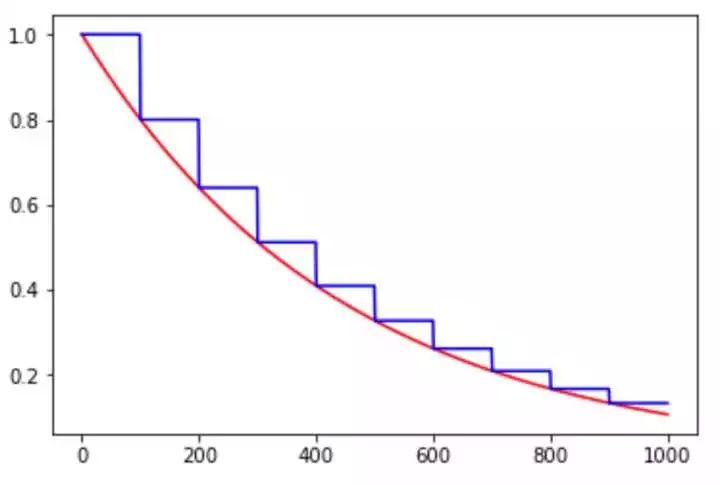
\includegraphics{./img/ch14/指数衰减.jpeg}
\caption{./}
\end{figure}

2、\textbf{piecewise\_constant}

\begin{Shaded}
\begin{Highlighting}[]
\NormalTok{piecewise_constant(x, boundaries, values, name}\OperatorTok{=}\VariableTok{None}\NormalTok{)}
\end{Highlighting}
\end{Shaded}

分段设置学习率法,跟指数型类似,区别在于每个阶段的衰减并不是按指数调整。可在不同阶段设置手动不同的学习率。这种学习率重点在有利于精调。

3、\textbf{polynomial\_decay}

\begin{Shaded}
\begin{Highlighting}[]
\NormalTok{polynomial_decay(learning_rate, global_step, decay_steps,}
\NormalTok{                  end_learning_rate}\OperatorTok{=}\FloatTok{0.0001}\NormalTok{, power}\OperatorTok{=}\FloatTok{1.0}\NormalTok{,}
\NormalTok{                  cycle}\OperatorTok{=}\VariableTok{False}\NormalTok{, name}\OperatorTok{=}\VariableTok{None}\NormalTok{)}
\end{Highlighting}
\end{Shaded}

多项式衰减,计算如下:

\[
global setp = min(global step, decay steps)
\]

\[
lr_{decayed} = (lr-lr_{end})*(1-{globalstep\over decaysteps})^{power} +lr_{end}
\]

有别于上述两种,多项式衰减则是在每一步迭代上都会调整学习率。主要看Power参数,若Power为1,则是下图中的红色直线;若power小于1,则是开1/power次方,为蓝色线;绿色线为指数,power大于1。

\begin{figure}
\centering
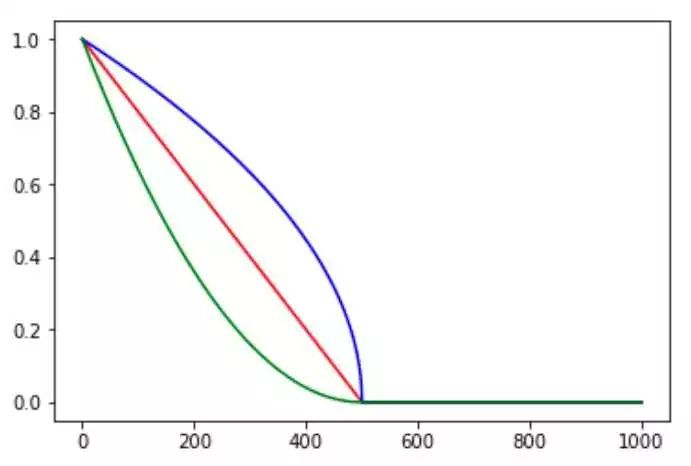
\includegraphics{./img/ch14/多项式衰减.jpeg}
\caption{}
\end{figure}

此外,需要注意的是参数cycle,cycle对应的是一种周期循环调整的方式。这种cycle策略主要目的在后期防止在一个局部极小值震荡,若跳出该区域或许能得到更有的结果。这里说明cycle的方式不止可以在多项式中应用,可配合类似的周期函数进行衰减,如下图。

\begin{figure}
\centering
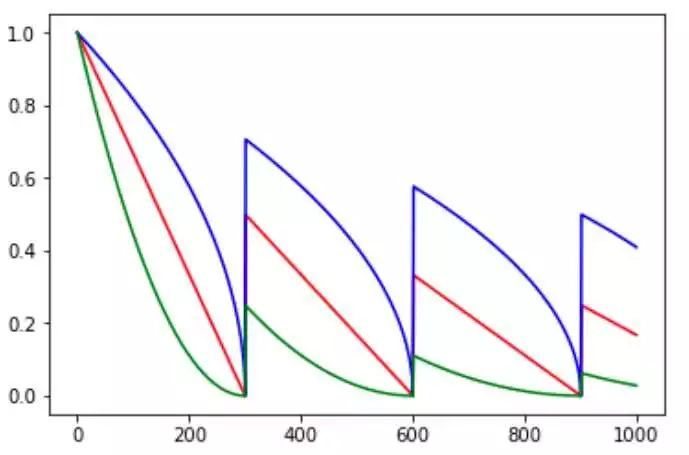
\includegraphics{./img/ch14/cycle衰减.jpeg}
\caption{}
\end{figure}

4、\textbf{inverse\_time\_decay}

\begin{Shaded}
\begin{Highlighting}[]
\NormalTok{inverse_time_decay(learning_rate, global_step, decay_steps, decay_rate,}
\NormalTok{                   staircase}\OperatorTok{=}\VariableTok{False}\NormalTok{, name}\OperatorTok{=}\VariableTok{None}\NormalTok{)}
\end{Highlighting}
\end{Shaded}

逆时衰减,这种方式和指数型类似。如图,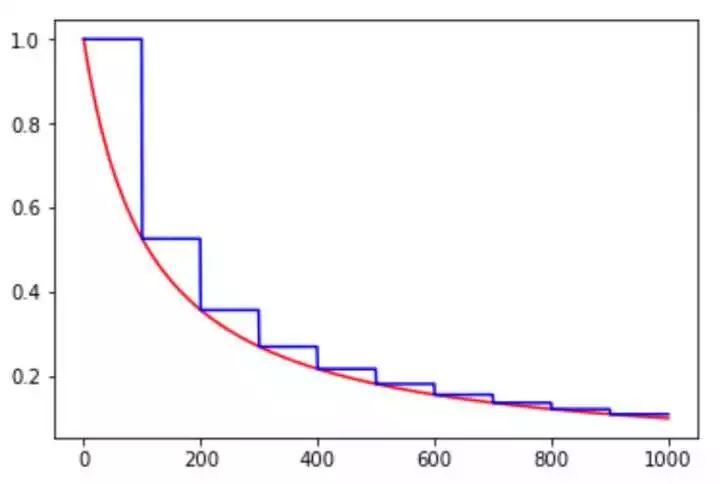
\includegraphics{./img/ch14/逆时衰减.jpeg}

5、\textbf{cosine\_decay}

\begin{Shaded}
\begin{Highlighting}[]
\NormalTok{cosine_decay(learning_rate, global_step, decay_steps, alpha}\OperatorTok{=}\FloatTok{0.0}\NormalTok{,}
\NormalTok{                 name}\OperatorTok{=}\VariableTok{None}\NormalTok{)}
\end{Highlighting}
\end{Shaded}

余弦衰减,即按余弦函数的方式衰减学习率,如图

\begin{figure}
\centering
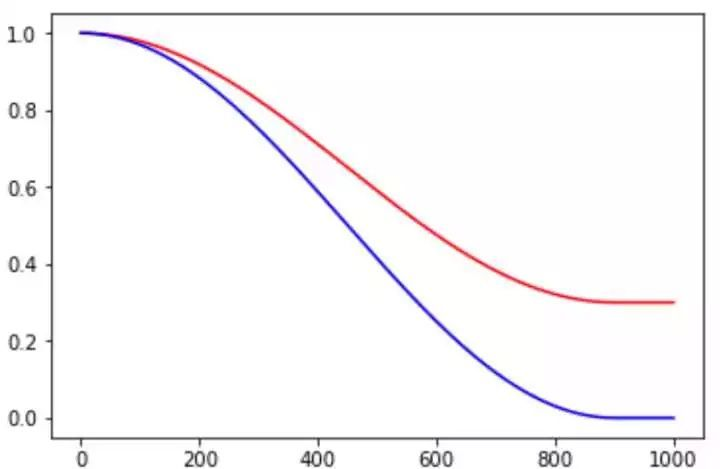
\includegraphics{./img/ch14/余弦衰减.jpeg}
\caption{}
\end{figure}

6、\textbf{cosine\_decay\_restarts}

\begin{Shaded}
\begin{Highlighting}[]
\NormalTok{cosine_decay_restarts(learning_rate, global_step, first_decay_steps,}
\NormalTok{                           t_mul}\OperatorTok{=}\FloatTok{2.0}\NormalTok{, m_mul}\OperatorTok{=}\FloatTok{1.0}\NormalTok{, alpha}\OperatorTok{=}\FloatTok{0.0}\NormalTok{, name}\OperatorTok{=}\VariableTok{None}\NormalTok{)}
\end{Highlighting}
\end{Shaded}

余弦衰减,即余弦版本的cycle策略,作用与多项式衰减中的cycle相同。区别在于余弦重启衰减会重新回到初始学习率,拉长周期,而多项式版本则会逐周期衰减。

\begin{figure}
\centering
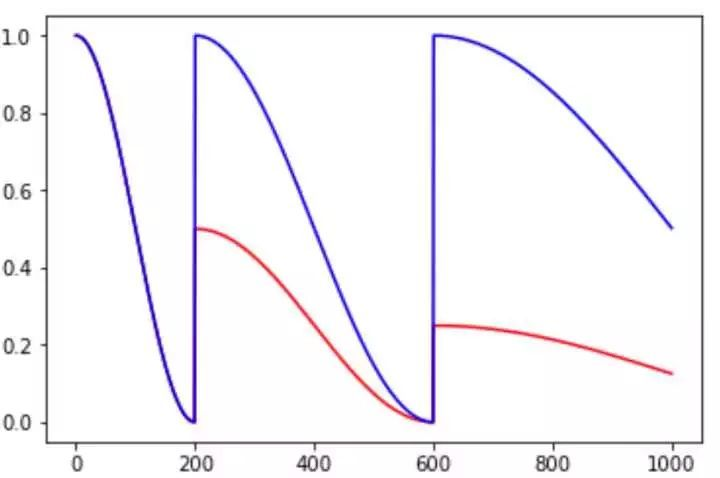
\includegraphics{./img/ch14/余弦cycle衰减.jpeg}
\caption{}
\end{figure}

7、\textbf{linear\_cosine\_decay}

\begin{Shaded}
\begin{Highlighting}[]
\NormalTok{linear_cosine_decay(learning_rate, global_step, decay_steps,}
\NormalTok{                        num_periods}\OperatorTok{=}\FloatTok{0.5}\NormalTok{, alpha}\OperatorTok{=}\FloatTok{0.0}\NormalTok{, beta}\OperatorTok{=}\FloatTok{0.001}\NormalTok{,}
\NormalTok{                        name}\OperatorTok{=}\VariableTok{None}\NormalTok{)}
\end{Highlighting}
\end{Shaded}

线性余弦衰减,主要应用于增强学习领域。

\begin{figure}
\centering
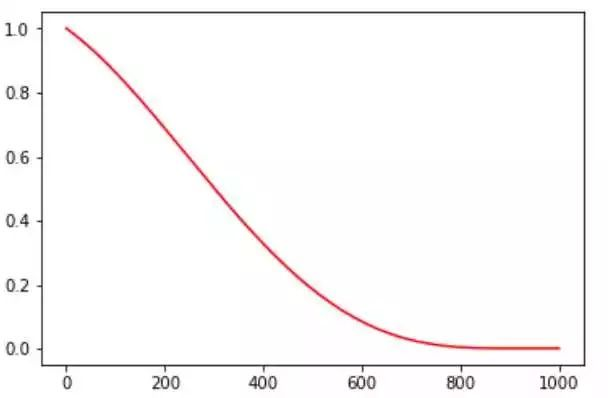
\includegraphics{./img/ch14/线性余弦衰减.jpeg}
\caption{}
\end{figure}

8、\textbf{noisy\_linear\_cosine\_decay}

噪声线性余弦衰减,即在线性余弦衰减中加入随机噪声,增大寻优的随机性。

\begin{figure}
\centering
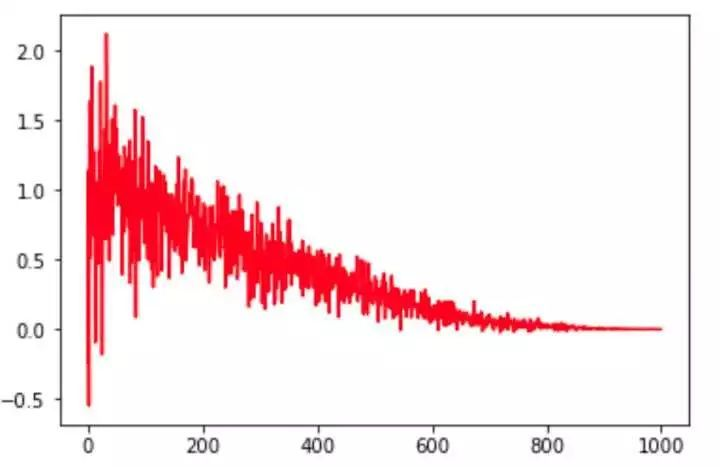
\includegraphics{./img/ch14/噪声线性余弦衰减.jpeg}
\caption{}
\end{figure}

\subsection{14.3.4
极端批样本数量下,如何训练网络?}\label{ux6781ux7aefux6279ux6837ux672cux6570ux91cfux4e0bux5982ux4f55ux8badux7ec3ux7f51ux7edc}

​ 极端批样本情况一般是指batch size为1或者batch
size在6000以上的情况。这两种情况,在使用不合理的情况下都会导致模型最终性能无法达到最优甚至是崩溃的情况。

​ 在目标检测、分割或者3D图像等输入图像尺寸较大的场景,通常batch size
会非常小。而在14.2.4中,我们已经讲到这种情况会导致梯度的不稳定以及batchnorm统计的不准确。针对梯度不稳定的问题,通常不会太致命,若训练中发现梯度不稳定导致性能的严重降低时可采用累计梯度的策略,即每次计算完不反向更新,而是累计多次的误差后进行一次更新,这是一种在内存有限情况下实现有效梯度更新的一个策略。batch
size过小通常对batchnorm的影响是最大的,若网络模型中存在batchnorm,batch
size若只为1或者2时会对训练结果产生非常大的影响。这时通常有两种策略,一、若模型使用了预训练网络,可冻结预训练网络中batchnorm的模型参数,有效降低batch
size引起的统计量变化的影响。二、在网络不是过深或者过于复杂时可直接移除batchnorm或者使用groupnorm代替batchnorm,前者不多阐释,后者是有FAIR提出的一种用于减少batch对batchnorm影响,其主要策略是先将特征在通道上进行分组,然后在组内进行归一化。即归一化操作上完全与batch
size无关。这种groupnorm的策略被证实在极小批量网络训练上能达到较优秀的性能。当然这里也引入里group这个超参数,一般情况下建议不宜取group为1或者各通道单独为组的group数量,可结合实际网络稍加调试。

​ 为了降低训练时间的成本,多机多卡的分布式系统通常会使用超大的batch
size进行网络训练。同样的在14.2.4中,我们提到了超大batch
size会带来梯度方向过于一致而导致的精度大幅度降低的问题。这时通常可采用层自适应速率缩放(LARS)算法。从理论认知上将,batch
size增大会减少反向传播的梯度更新次数,但为了达到相同的模型效果,需要增大学习率。但学习率一旦增大,又会引起模型的不收敛。为了解决这一矛盾,LARS算法就在各层上自适应的计算一个本地学习率用于更新本层的参数,这样能有效的提升训练的稳定性。目前利用LARS算法,腾讯公司使用65536的超大batch
size能将ResNet50在ImageNet在4分钟完成训练,而谷歌使用32768的batch
size使用TPU能将该时间缩短至2分钟。

\section{14.4
合理使用预训练网络}\label{ux5408ux7406ux4f7fux7528ux9884ux8badux7ec3ux7f51ux7edc}

\subsection{14.4.1
什么是微调(fine-tune)}\label{ux4ec0ux4e48ux662fux5faeux8c03fine-tune}

​
微调(fine-tune),顾名思义指稍微调整参数即可得到优秀的性能,是迁移学习的一种实现方式。微调和从头训练(train
from scratch)的本质区别在于模型参数的初始化,train from
scratch通常指对网络各类参数进行随机初始化(当然随机初始化也存在一定技巧),随机初始化模型通常不具有任何预测能力,通常需要大量的数据或者特定域的数据进行从零开始的训练,这样需要训练到优秀的模型通常是稍困难的。而微调的网络,网络各类参数已经在其他数据集(例如ImageNet数据集)完成较好调整的,具备了较优秀的表达能力。因此,我们只需要以较小的学习速率在自己所需的数据集领域进行学习即可得到较为优秀的模型。微调通常情况下,无须再重新设计网络结构,预训练模型提供了优秀的结构,只需稍微修改部分层即可。在小数据集上,通常微调的效果比从头训练要好很多,原因在于数据量较小的前提下,训练更多参数容易导致过度拟合。

\subsection{14.4.2
微调有哪些不同方法?}\label{ux5faeux8c03ux6709ux54eaux4e9bux4e0dux540cux65b9ux6cd5}

​
以图像分类为例,通常情况下由于不同数据集需要的类别数不同,我们需要修改网络的输出顶层。这种情况下有两种微调方式:

\begin{itemize}
\item
  不冻结网络模型的任何层,对最后的改动层使用较大的学习率,对未改动层以较小的学习率进行训练全模型训练,进行多轮训练即可。即一步完成训练。
\item
  冻结除了顶部改动层以外的所有层参数,即不对冻结部分的层进行参数训练更新,进行若干轮的微调训练后,放开顶部层以下的若干层或者全部放开所有层的参数,再次进行若干轮训练即可。即分多步训练。
\end{itemize}

以上两种都属于微调。目前由于存在大量优秀的预训练模型,如何确定哪个模型适合自己的任务并能得到最佳性能需要花大量的时间探索。此时,上述的前者是种不错训练方式,你无须进行过多分步的操作。而当探索到一个比较适合的模型时,你不妨可以再次重新尝试下以第二种方式进行训练,或许能得到相比于前者稍高些的性能,因为小数据集上调整过多的参数过拟合的机率也会增大,当然这并不是绝对的。

\subsection{14.4.3
微调先冻结底层,训练顶层的原因?}\label{ux5faeux8c03ux5148ux51bbux7ed3ux5e95ux5c42ux8badux7ec3ux9876ux5c42ux7684ux539fux56e0}

​
14.12中第二种冻结多步训练的方式。首先冻结除了顶部改动层以外的所有层参数,对顶层进行训练,这个过程可以理解为顶层的域适应训练,主要用来训练适应模型的现有特征空间,防止顶层糟糕的初始化,对已经具备一定表达能力的层的干扰和破坏,影响最终的性能。之后,在很多深度学习框架教程中会使用放开顶层往下一半的层数,继续进行微调。这样的好处在于越底层的特征通常是越通用的特征,越往上其整体的高层次语义越完备,这通过感受野很容易理解。所以,若预训练模型的数据和微调训练的数据语义差异越大(例如ImageNet的预模型用于医学图像的训练),那越往顶层的特征语义差异就越大,因此通常也需要进行相应的调整。

\subsection{14.4.4
不同的数据集特性下如何微调?}\label{ux4e0dux540cux7684ux6570ux636eux96c6ux7279ux6027ux4e0bux5982ux4f55ux5faeux8c03}

\begin{itemize}
% \tightlist
\item
  数据集数据量少,数据和原数据集类似。这是通常做法只需修改最后的输出层,训练即可,训练过多参数容易过拟合。
\item
  数据集数据量少,数据和原数据集差异较大。由于数据差异较大,可以在完成输出顶层的微调后,微调顶层往下一半的层数,进行微调。
\item
  数据集数据量大,数据与原数据集差异较大。这种情况下,通常已经不需要用预训练模型进行微调,通常直接重新训练即可。
\item
  数据集数据量大,数据与原数据类似。这时预训练模型的参数是个很好的初始化,可利用预训练模型放开所有层以较小的学习率微调即可。
\end{itemize}

\subsection{14.4.4
目标检测中使用预训练模型的优劣?}\label{ux76eeux6807ux68c0ux6d4bux4e2dux4f7fux7528ux9884ux8badux7ec3ux6a21ux578bux7684ux4f18ux52a3}

​ 目标检测中无论是一阶段的YOLO、SSD或者RetinaNet 还是二阶段的Faster
R-CNN、R-FCN 和 FPN都是基于ImageNet上预训练好的分类模型。

​ 优势在于:

​
1、正如大部分微调的情况一样,使用预训练网络已拥有优秀的语义特征,能有效的加快训练速度;

​
2、其次,对于大部分二阶段的模型来说,并未实现严格意义上的完全端对端的训练,所以使用预训练模型能直接提取到语义特征,能使两个阶段的网络更容易实现模型的优化。

​ 劣势在于,分类模型和检测模型之间仍然存在一定任务上的差异:

​
1、分类模型大部分训练于单目标数据,对同时进行多目标的捕捉能力稍弱,且不关注目标的位置,在一定程度上让模型损失部分空间信息,这对检测模型通常是不利的;

​
2、域适应问题,若预训练模型(ImageNet)和实际检测器的使用场景(医学图像,卫星图像)差异较大时,性能会受到影响;

​ 3、使用预训练模型就意味着难以自由改变网络结构和参数限制了应用场合。

\subsection{14.4.5 目标检测中如何从零开始训练(train from
scratch)?}\label{ux76eeux6807ux68c0ux6d4bux4e2dux5982ux4f55ux4eceux96f6ux5f00ux59cbux8badux7ec3train-from-scratch}

​
结合FAIR相关的研究,我们可以了解目标检测和其他任务从零训练模型一样,只要拥有足够的数据以及充分而有效的训练,同样能训练出不亚于利用预训练模型的检测器。这里我们提供如下几点建议:

​ 1、数据集不大时,同样需要进行数据集增强。

​ 2、预训练模型拥有更好的初始化,train from
scratch需要更多的迭代次数以及时间训练和优化检测器。而二阶段模型由于并不是严格的端对端训练,此时可能需要更多的迭代次数以及时间,而一阶段检测模型训练会相对更容易些(例如DSOD以ScratchDet及)。

​ 3、目标检测中train from scratch最大的问题还是batch
size过小。所以可采取的策略是增加GPU使用异步batchnorm增大batch
size,若条件限制无法使用更多GPU时,可使用groupnorm代替batchnorm

​
4、由于分类模型存在对多目标的捕捉能力弱以及对物体空间位置信息不敏感等问题,可借鉴DetNet训练一个专属于目标检测的模型网络,增强对多目标、尺度和位置拥有更强的适应性。

\section{14.5 如何改善 GAN
的性能}\label{ux5982ux4f55ux6539ux5584-gan-ux7684ux6027ux80fd}

优化GAN性能通常需要在如下几个方面进行

\begin{itemize}
% \tightlist
\item
  设计或选择更适合目的代价函数。
\item
  添加额外的惩罚。
\item
  避免判别器过度自信和生成器过度拟合。
\item
  更好的优化模型的方法。
\item
  添加标签明确优化目标。
\end{itemize}

GAN常用训练技巧

\begin{itemize}
\item
  输入规范化到(-1,1)之间,最后一层的激活函数使用tanh(BEGAN除外)
\item
  使用wassertein GAN的损失函数,
\item
  如果有标签数据的话,尽量使用标签,也有人提出使用反转标签效果很好,另外使用标签平滑,单边标签平滑或者双边标签平滑
\item
  使用mini-batch norm, 如果不用batch norm 可以使用instance norm
  或者weight norm
\item
  避免使用RELU和pooling层,减少稀疏梯度的可能性,可以使用leakrelu激活函数
\item
  优化器尽量选择ADAM,学习率不要设置太大,初始1e-4可以参考,另外可以随着训练进行不断缩小学习率,
\item
  给D的网络层增加高斯噪声,相当于是一种正则 \#\# 14.6 AutoML
\end{itemize}

\subsection{14.6.1 什么是AutoML?}\label{ux4ec0ux4e48ux662fautoml}

​ 目前一个优秀的机器学习和深度学习模型,离不开这几个方面:

​ 一、优秀的数据预处理;

​ 二、合适的模型结构和功能;

​ 三、优秀的训练策略和超参数;

​ 四、合适的后处理操作;

​ 五、严格的结果分析。

​
这几方面都对最终的结果有着举足轻重的影响,这也是目前的数据工程师和学者们的主要工作。但由于这每一方面都十分繁琐,尤其是在构建模型和训练模型上。而大部分情况下,这些工作有无须过深专业知识就能使用起来。所以AutoML主要的作用就是来帮助实现高效的模型构建和超参数调整。例如深度学习网络的架构搜索、超参数的重要性分析等等。当然AutoML并不简单的进行暴力或者随机的搜索,其仍然需要机器学习方面的知识,例如贝叶斯优化、强化学习、元学习以及迁移学习等等。目前也有些不错的AutoML工具包,例如Alex
Honchar的Hyperopt、微软的NNI、Autokeras等。

目前AutoML已经成为最新的研究热点,有兴趣的可以参考\href{https://www.automl.org/automl/literature-on-neural-architecture-search/}{AutoML
literature}。

\subsection{14.6.2
自动化超参数搜索方法有哪些?}\label{ux81eaux52a8ux5316ux8d85ux53c2ux6570ux641cux7d22ux65b9ux6cd5ux6709ux54eaux4e9b}

​ 目前自动化搜索主要包含网格搜索,随机搜索,基于模型的超参优化

​ 网格搜索:

​
通常当超参数量较少的时候,可以使用网格搜索法。即列出每个超参数的大致候选集合。利用这些集合
进行逐项组合优化。在条件允许的情况下,重复进行网格搜索会当优秀,当然每次重复需要根据上一步得到的最优参数组合,进行进一步的细粒度的调整。网格搜索最大的问题就在于计算时间会随着超参数的数量指数级的增长。

​ 随机搜索:

​
随机搜索,是一种用来替代网格搜索的搜索方式。随机搜索有别于网格搜索的一点在于,我们不需要设定一个离散的超参数集合,而是对每个超参数定义一个分布函数来生成随机超参数。随机搜索相比于网格搜索在一些不敏感超参上拥有明显优势。例如网格搜索对于批样本数量(batch
size),在{[}16,32,64{]}这些范围内进行逐项调试,这样的调试显然收益更低下。当然随机搜索也可以进行细粒度范围内的重复的搜索优化。

\begin{figure}
\centering
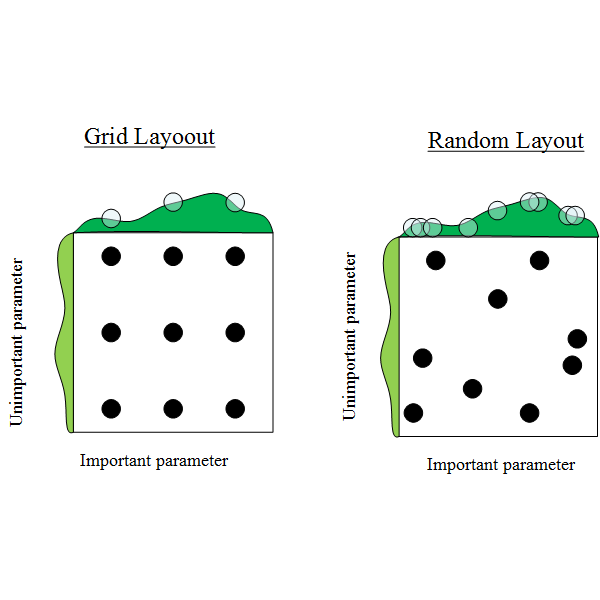
\includegraphics{./img/ch14/14.14.png}
\caption{}
\end{figure}

​ 基于模型的超参优化:

​
有别于上述两种的搜索策略,基于模型的超参调优问题转化为了优化问题。直觉上会考虑是否进行一个可导建模,然后利用梯度下降进行优化。但不幸的是我们的超参数通常情况下是离散的,而且其计算代价依旧很高。

​
基于模型的搜索算法,最常见的就是贝叶斯超参优化。有别于的网格搜索和随机搜索独立于前几次搜索结果的搜索,贝叶斯则是利用历史的搜索结果进行优化搜索。其主要有四部分组成,1.目标函数,大部分情况下就是模型验证集上的损失。2、搜索空间,即各类待搜索的超参数。3、优化策略,建立的概率模型和选择超参数的方式。4、历史的搜索结果。首先对搜索空间进行一个先验性的假设猜想,即假设一种选择超参的方式,然后不断的优化更新概率模型,最终的目标是找到验证集上误差最小的一组超参数。

\subsection{14.6.3
什么是神经网络架构搜索(NAS)}\label{ux4ec0ux4e48ux662fux795eux7ecfux7f51ux7edcux67b6ux6784ux641cux7d22nas}

2015至2017年间,是CNN网络设计最兴盛的阶段,大多都是由学者人工设计的网络结构。这个过程通常会很繁琐。其主要原因在于对不同模块组件的组成通常是个黑盒优化的问题,此外,在不同结构超参数以及训练超参数的选择优化上非凸优化问题,或者是个混合优化问题,既有离散空间又有连续空间。NAS(Neural
Architecture
Search)的出现就是为了解决如何通过机器策略和自动化的方式设计出优秀高效的网络。而这种策略通常不是统一的标准,不同的网络结合实际的需求通常会有不同的设计,比如移动端的模型会在效率和精度之间做平衡。目前,NAS也是AUTOML中最重要的部分。NAS通常会分为三个方面,搜索空间(在哪搜索),搜索策略(如何搜索)及评价预估。

\begin{itemize}
\item
  搜索空间,即在哪搜索,定义了优化问题所需变量。不同规模的搜索空间的变量其对于的难度也是不一样的。早期由于网络结构以及层数相对比较简单,参数量较少,因此会更多的使用遗传算法等进化算法对网络的超参数和权重进行优化。深度学习发展到目前,模型网络结构越来越复杂,参数量级越来越庞大,这些进化算法已经无法继续使用。但若我们先验给定一些网络结构和超参数,模型的性能已经被限制在给定的空间,此时搜索的空间已变得有限,所以只需对复杂模型的架构参数和对应的超参数进行优化即可。
\item
  搜索策略,
  即如何搜索,定义了如何快速、准确找到最优的网络结构参数配置的策略。常见的搜索方法包括:随机搜索、贝叶斯优化、强化学习、进化算法以及基于模型的搜索算法。其中主要代表为2017年谷歌大脑的使用强化学习的搜索方法。
\item
  评价预估,定义了如何高效对搜索的评估策略。深度学习中,数据规模往往是庞大的,模型要在如此庞大的数据规模上进行搜索,这无疑是非常耗时的,对优化也会造成非常大的困难,所以需要一些高效的策略做近似的评估。
  这里一般会有如下三种思路:
\end{itemize}

一、使用些低保真的训练集来训练模型。低保真在实际中可以用不同的理解,比如较少的迭代次数,用一小部分数据集或者保证结构的同时减少通道数等。这些方法都可以在测试优化结构时大大降低计算时间,当然也会存在一定的偏差。但架构搜索从来并不是要一组固定的参数,而是一种优秀的模型结构。最终选取时,只需在较优秀的几组结构中进行全集训练,进行择优选取即可。

二、使用代理模型。除了低保真的训练方式外,学者们提出了一种叫做代理模型的回归模型,采用例如插值等策略对已知的一些参数范围进行预测,目的是为了用尽可能少的点预测到最佳的结果。

三、参数级别的迁移。例如知识蒸馏等。用已训练好的模型权重参数对目标问题搜索,通常会让搜索拥有一个优秀的起点。由于积累了大量的历史寻优数据,对新问题的寻优将会起到很大的帮助。

\subsection{14.6.4
NASNet的设计策略}\label{nasnetux7684ux8bbeux8ba1ux7b56ux7565}

NASNet是最早由google brain
通过网络架构搜索策略搜索并成功训练ImageNet的网络,其性能超越所有手动设计的网络模型。关于NASNet的搜索策略,首先需要参考google
brain发表在ICLR2017的论文《Neural Architecture Search with Reinforcement
Learning》。该论文是最早成功通过架构搜索策略在cifar-10数据集上取得比较不错效果的工作。NASNet很大程度上是沿用该搜索框架的设计思想。

NASNet的核心思想是利用强化学习对搜索空间内的结构进行反馈探索。架构搜索图如下,定义了一个以RNN为核心的搜索控制器。在搜索空间以概率p对模型进行搜索采样。得到网络模型A后,对该模型进行训练,待模型收敛得到设定的准确率R后,将梯度传递给控制器RNN进行梯度更新。

\begin{figure}
\centering
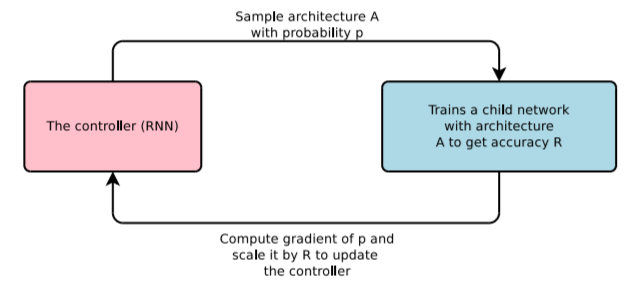
\includegraphics{./img/ch14/NAS搜索策略.png}
\caption{}
\end{figure}

​ 架构搜索策略流程

RNN控制器会对卷积层的滤波器的尺寸、数量以及滑动间隔进行预测。每次预测的结果都会作为下一级的输入,档层数达到设定的阈值时,会停止预测。而这个阈值也会随着训练的进行而增加。这里的控制器之预测了卷积,并没有对例如inception系列的分支结构或者ResNet的跳级结构等进行搜索。所以,控制器需要进一步扩展到预测这些跳级结构上,这样搜索空间相应的也会增大。为了预测这些结构,RNN控制器内每一层都增加了一个预测跳级结构的神经元,文中称为锚点,稍有不同的是该锚点的预测会由前面所有层的锚点状态决定。

\begin{figure}
\centering
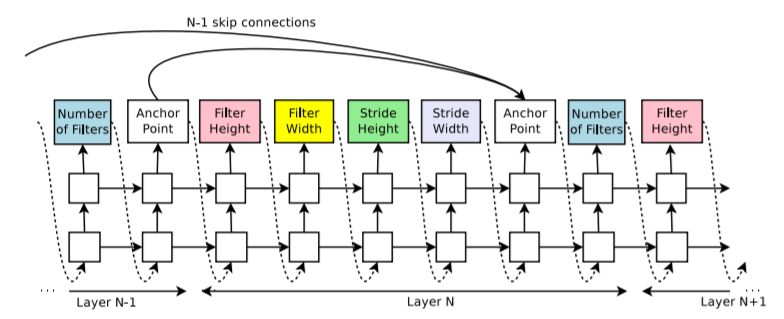
\includegraphics{./img/ch14/RNN控制器.png}
\caption{}
\end{figure}

​ RNN控制器

NASNet大体沿用了上述生成网络结构的机器,并在此基础上做了如下两点改进:

1、先验行地加入inception系列和ResNet的堆叠模块的思想。其定义了两种卷积模块,Normal
Cell和Reduction
Cell,前者不进行降采样,而后者是个降采样的模块。而由这两种模块组成的结构可以很方便的通过不同数量的模块堆叠将其从小数据集搜索到的架构迁移到大数据集上,大大提高了搜索效率。

\begin{figure}
\centering
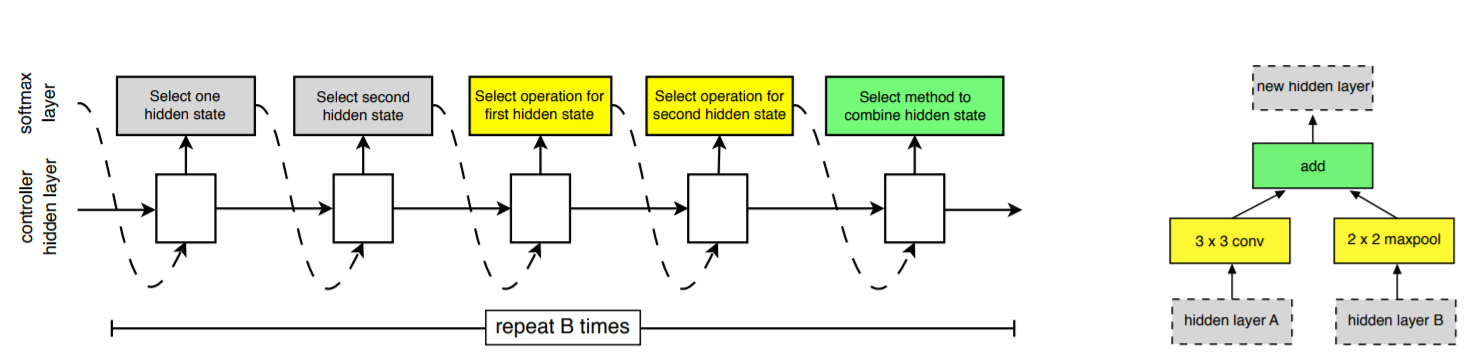
\includegraphics{./img/ch14/NASNet的RNN控制器.png}
\caption{}
\end{figure}

​ NASNet的RNN控制器

2、对RNN控制进行优化,先验性地将各种尺寸和类型的卷积和池化层加入到搜索空间内,用预测一个卷积模块代替原先预测一层卷积。如图,控制器RNN不在预测单个卷积内的超参数组成,而是对一个模块内的每一个部分进行搜索预测,搜索的空间则限定在如下这些操作中:

​ • identity • 1x3 then 3x1 convolution ​ • 1x7 then 7x1 convolution •
3x3 dilated convolution ​ • 3x3 average pooling • 3x3 max pooling ​ •
5x5 max pooling • 7x7 max pooling ​ • 1x1 convolution • 3x3 convolution
​ • 3x3 depthwise-separable conv • 5x5 depthwise-seperable conv ​ • 7x7
depthwise-separable conv

在模块内的连接方式上也提供了element-wise
addition和concatenate两种方式。NASNet的搜索方式和过程对NAS的一些后续工作都具有非常好的参考借鉴意义。

\subsection{14.6.5
网络设计中,为什么卷积核设计尺寸都是奇数}\label{ux7f51ux7edcux8bbeux8ba1ux4e2dux4e3aux4ec0ux4e48ux5377ux79efux6838ux8bbeux8ba1ux5c3aux5bf8ux90fdux662fux5947ux6570}

我们发现在很多大部分网络设计时都会使用例如3x3/5x5/7x7等奇数尺寸卷积核,主要原因有两点:

\begin{itemize}
% \tightlist
\item
  保证像素点中心位置,避免位置信息偏移
\item
  填充边缘时能保证两边都能填充,原矩阵依然对称
\end{itemize}

\subsection{14.6.6
网络设计中,权重共享的形式有哪些,为什么要权重共享}\label{ux7f51ux7edcux8bbeux8ba1ux4e2dux6743ux91cdux5171ux4eabux7684ux5f62ux5f0fux6709ux54eaux4e9bux4e3aux4ec0ux4e48ux8981ux6743ux91cdux5171ux4eab}

权重共享的形式:

\begin{itemize}
% \tightlist
\item
  深度学习中,权重共享最具代表性的就是卷积网络的卷积操作。卷积相比于全连接神经网络参数大大减少;
\item
  多任务网络中,通常为了降低每个任务的计算量,会共享一个骨干网络。
\item
  一些相同尺度下的结构化递归网络
\end{itemize}

权重共享的好处:

​
权重共享一定程度上能增强参数之间的联系,获得更好的共性特征。同时很大程度上降低了网络的参数,节省计算量和计算所需内存(当然,结构化递归并不节省计算量)。此外权重共享能起到很好正则的作用。正则化的目的是为了降低模型复杂度,防止过拟合,而权重共享则正好降低了模型的参数和复杂度。

​
因此一个设计优秀的权重共享方式,在降低计算量的同时,通常会较独享网络有更好的效果。

权重共享不仅在人工设计(human-invented)的网络结构中有简化参数,降低模型复杂度的作用,在神经网络搜索(NAS)的网络结构中可以使得child
model的计算效率提升,使得搜索过程可以在单卡GPU上复现,见Efficient
NAS(\href{https://arxiv.org/abs/1802.03268}{ENAS})。
